% Supporting theory and exact methods. The main document invokes \appendix.
\section{Supporting Mathematical Statements}\label{app:theory}

The statements in this appendix make the interpretation of the experiments
precise. They are elementary supporting results; we do not claim a new
KAHM approximation theorem. All conditional expectations below are understood
up to almost-sure equality. For scalar square-integrable $Y$, write
$m(X)=\E[Y\mid X]$ and
$R_X^{\mathrm{Bayes}}=\E[(Y-m(X))^2]$.
When a representation has been learned from independent training data,
the statements apply conditionally on that fitted representation.

\begin{proposition}[Information retained by a representation]
\label{prop:representation-risk}
For a measurable representation $U=\Gamma(X)$,
\[
 R_U^{\mathrm{Bayes}}-R_X^{\mathrm{Bayes}}
 =\E[(m(X)-\E[m(X)\mid U])^2].
\]
For any square-integrable prediction $f(U)$,
\[
 R(f\circ\Gamma)-R_X^{\mathrm{Bayes}}
 =\|m-f\circ\Gamma\|_{L^2}^2.
\]
\end{proposition}
\begin{proof}
Write $Y-f(U)=(Y-m(X))+(m(X)-f(U))$.
The cross term has expectation zero after conditioning on $X$.
Minimizing the second term over $U$-measurable predictions gives the
conditional expectation $\E[m(X)\mid U]$.
\end{proof}

\begin{proposition}[Restoring the outer score normalizer]
\label{prop:normalizer-inverse}
Let $T_1,\ldots,T_C\in[0,1]$, $\omega>0$, and $\tau>0$. Define
\[
 \ell_c=\omega\log(1-T_c+\tau),\qquad
 z=\log\sum_{j=1}^{C}\exp(\ell_j),\qquad
 \phi_c=\exp(\ell_c-z).
\]
Then $T$ and $(\phi,z)$ generate the same information in exact arithmetic,
and
\[
 T_c=1+\tau-\exp\{(\log\phi_c+z)/\omega\}.
\]
For multiple separately normalized blocks, one $z$ is required per block.
\end{proposition}
\begin{proof}
Strict positivity of $1-T_c+\tau$ implies $\phi_c>0$.
Hence $\log\phi_c+z=\ell_c$, which gives the inverse.
Both directions are measurable. Applying this argument to each block
gives the multiple-block statement.
\end{proof}

If scores are clipped before normalization, the inverse restores the
clipped scores. It does not restore discarded reconstruction vectors or
guarantee equal finite-head performance. In particular, the inverse is
nonlinear, so affine function classes on $T$ and on $(\phi,z)$ need not
coincide. This proposition concerns the outer association normalizer,
not the signed denominator in the KAHM reconstruction.

\begin{proposition}[A sufficient condition for an injective local code]
\label{prop:local-injectivity}
Fix a fitted bank with bases $P_c$ and centers $\mu_c$. Suppose its gates
are measurable and strictly positive, and let $A$ be the matrix obtained by vertically
stacking the matrices $P_c^\top$. If $A$ has full column rank $d$, then
\[
 z\longmapsto
 \left[\phi(z),\{\phi_c(z)P_c^\top(z-\mu_c)\}_c\right]
\]
is injective. In particular, this code and $z$ generate the same
information, and their Bayes risks agree for every square-integrable
target.
\end{proposition}
\begin{proof}
The code contains both $\phi_c(z)>0$ and its product with
$P_c^\top(z-\mu_c)$. Division and addition of the fixed vector
$P_c^\top\mu_c$ recover $P_c^\top z$ for every $c$. Stacking these
vectors gives $Az$. Full column rank gives the measurable inverse
$z=(A^\top A)^{-1}A^\top(Az)$. Conversely, the code is a measurable
function of $z$, so the generated information and Bayes risks agree.
\end{proof}

The gates in Equation~\eqref{eq:phi} are strictly positive in exact
arithmetic because $\tau>0$. The rank assumption is a sufficient
condition, not a necessary one: when $A$ is rank deficient, the gates
themselves may retain additional information. It must be checked for
each fitted bank. Very small gates and an ill-conditioned $A$ can make
the displayed inverse numerically unstable, and its existence does not
make it accessible to every finite decoder or fitting procedure.

\begin{proposition}[A score symmetry and its prediction consequence]
\label{prop:exact-symmetry}
Let $Q$ be orthogonal on a preprocessed input space. Suppose that each
group's reconstruction obeys $r_c(Qx)=Qr_c(x)$ and that $Q$ preserves
group identities. The radial--angular score in Section~\ref{sec:method},
its block affinities, and the block log normalizer are invariant under $Q$.

For the branch law in Equation~\eqref{eq:branch}, let
$Q(x_1,x_2)=(-x_1,x_2)$. Any representation $U=\Gamma(X)$ satisfying
$\Gamma(QX)=\Gamma(X)$ almost surely has
\[
 R_U^{\mathrm{Bayes}}
 =\frac{1}{300}+\lambda
  +(1-\lambda)\E[(S-\E[S\mid U])^2].
\]
Consequently $R_U^{\mathrm{Bayes}}\geq 1/300+\lambda$, with equality
when $U$ determines $S$.
\end{proposition}
\begin{proof}
Orthogonality preserves norms and inner products, including the zero-norm
convention for the angle. Equivariance therefore preserves each radial
and angular discrepancy, hence its combined score. Block normalization
and its log normalizer are deterministic functions of those scores.

For the branch law, replacing $T$ by $-T$ leaves the joint distribution
of $(S,T)$ unchanged and leaves $U$ unchanged. Thus $\E[T\mid U]=0$.
Also $S$ is even under this reflection, whereas $T$ is odd. It follows
that $\E[(S-\E[S\mid U])T]=0$. Expanding the square in
Proposition~\ref{prop:representation-risk}, using
$\E[T^2]=1/3$ and $\Var(\epsilon)=1/300$, yields the displayed identity.
\end{proof}

The first assertion also holds when $Q$ permutes reconstructors within a
group whose score is their minimum. Permuting distinct groups, however,
can permute the affinity coordinates rather than leaving the representation
unchanged. Nor does a raw-input reflection necessarily commute with a
training-fitted scaler. Finite learned partitions and reference sets need
not satisfy the proposition's assumptions. The measured near-invariance
of one learned code is therefore a diagnostic, not a proof that its
Bayes risk equals the exact-symmetry lower bound. Tiny nonzero differences
could in principle be used by an unrestricted decoder.

\begin{proposition}[Approximate symmetry under a decoder budget]
\label{prop:approx-symmetry}
Let $Q$ be a measurable, distribution-preserving involution on the input
space: $Q^2X=X$ almost surely and $QX$ has the law of $X$.
Let $d_U$ be a measurable pseudometric on the representation space and
$g$ be $\kappa$-Lipschitz for this pseudometric. Assume
$m,g\circ\Gamma\in L^2$ and
\[
 \delta_\Gamma^2
 =\E[d_U(\Gamma(X),\Gamma(QX))^2]<\infty.
\]
With $m_o=(m-m\circ Q)/2$,
\[
 R(g\circ\Gamma)-R_X^{\mathrm{Bayes}}
 \geq (\|m_o\|_{L^2}-\kappa\delta_\Gamma/2)_+^2.
\]
For the branch law, $\|m_o\|_{L^2}=\sqrt\lambda$.
\end{proposition}
\begin{proof}
The operator $Vh=h\circ Q$ is an isometric involution on $L^2(P_X)$.
The even and odd components $h_e=(h+Vh)/2$ and $h_o=(h-Vh)/2$
are orthogonal. In particular, with $f=g\circ\Gamma$,
\[
 \|m-f\|_{L^2}^2
 =\|m_e-f_e\|_{L^2}^2+\|m_o-f_o\|_{L^2}^2
 \geq\|m_o-f_o\|_{L^2}^2.
\]
The Lipschitz condition gives
$|f_o(X)|\leq\kappa d_U(\Gamma(X),\Gamma(QX))/2$, so
$\|f_o\|_{L^2}\leq\kappa\delta_\Gamma/2$.
Apply the reverse triangle inequality and
Proposition~\ref{prop:representation-risk}.
For the branch law, $m_o(X)=\sqrt{3\lambda}\,T$ and
$\E[T^2]=1/3$.
\end{proof}

An empirical reflection distance is not automatically a population upper
bound for $\delta_\Gamma$. A valid numerical lower bound obtained from
this proposition would need uncertainty control in that direction and a
verified decoder Lipschitz constant for the same metric. Neither is
asserted for the experiment's unconstrained diagnostic heads.

\begin{proposition}[Reconstruction through the predictor's representation]
\label{prop:reconstruction-bridge}
Suppose a version of $m$ is $L$-Lipschitz on a domain containing $X$ and
$h(U)$ almost surely, and
$\E\|X-h(U)\|_2^2\leq\varepsilon_{\mathrm{rec}}^2$.
Then
\[
 R_U^{\mathrm{Bayes}}-R_X^{\mathrm{Bayes}}
 \leq L^2\varepsilon_{\mathrm{rec}}^2.
\]
If $h$ is additionally $L_h$-Lipschitz from the declared representation
metric and $\kappa\geq LL_h$, the same upper bound applies to the
infimum excess risk over $\kappa$-Lipschitz decoders:
\[
 \inf_{\operatorname{Lip}(g)\leq\kappa}
 \{R(g\circ\Gamma)-R_X^{\mathrm{Bayes}}\}
 \leq L^2\varepsilon_{\mathrm{rec}}^2.
\]
If a particular decoder
$f$ instead satisfies
$\|m\circ h-f\|_{L^2(P_U)}\leq\delta_{\mathrm{head}}$, then
\[
 R(f\circ\Gamma)-R_X^{\mathrm{Bayes}}
 \leq (L\varepsilon_{\mathrm{rec}}+\delta_{\mathrm{head}})^2.
\]
\end{proposition}
\begin{proof}
Conditional expectation is the $L^2$ projection onto the
$U$-measurable functions. The admissible prediction $m(h(U))$ gives
\[
 \E[(m(X)-\E[m(X)\mid U])^2]
 \leq \E[(m(X)-m(h(U)))^2]
 \leq L^2\E\|X-h(U)\|_2^2.
\]
For the constrained statement, $m\circ h$ has Lipschitz constant at
most $LL_h$. For a particular $f$, the triangle inequality in $L^2$
gives $\|m-f\circ\Gamma\|_{L^2}
\leq L\varepsilon_{\mathrm{rec}}+\delta_{\mathrm{head}}$.
Use Proposition~\ref{prop:representation-risk} in each case.
\end{proof}

The essential assumption is the existence of $h$ as a function of the
retained representation. A KAHM reconstruction evaluated on the raw query
is not such a function merely because its residual is small. The domain
assumption also matters: a conditional mean initially defined only on the
support of $X$ must have the specified Lipschitz version at $h(U)$.

\begin{proposition}[Common scaling of an inner kernel row]
\label{prop:inner-scaling}
Let $k$ be a finite kernel row, let $B$ be the fixed fitted matrix, and
suppose $kB\boldsymbol 1\ne0$. For every real $a>0$,
\[
 \frac{akB}{akB\boldsymbol 1}
 =\frac{kB}{kB\boldsymbol 1}.
\]
Thus evaluating a Gaussian query row by
$\exp(\ell_j-\max_i\ell_i)$ preserves its normalized signed weights
in exact arithmetic whenever the original denominator is nonzero.
\end{proposition}
\begin{proof}
The common factor cancels from numerator and denominator.
For finite log-kernel values, the centered exponential row is the
original row times $a=\exp(-\max_i\ell_i)>0$ in real arithmetic.
\end{proof}

This statement neither rescales the training kernel nor permits replacing
$B$. It does not address a genuinely zero signed denominator or prevent
cancellation. The purpose of the implemented change is to avoid evaluating
an entire query row as floating-point zero before normalization.

\section{Generators, Shared Components, and Decoders}\label{app:methods}

\subsection{Exact forecasting laws and target construction}

The nonlinear AR generator starts with independent
$u_0,u_1\sim\mathrm{Unif}[-0.8,0.8]$ and uses
\[
 u_{t+1}=\tanh\{1.25u_t-0.65u_{t-1}
                   +0.25\sin(3u_t)+\eta_{t+1}\},
 \qquad\eta_t\stackrel{\mathrm{iid}}\sim\mathrm{Unif}[-0.1,0.1].
\]
The first 80 stored values are discarded; the next 72 are the episode.
Each episode uses an independent initial state and innovation sequence.

The Van der Pol and Duffing systems respectively use
\begin{align*}
 \dot x&=v,& \dot v&=(1-x^2)v-x,\\
 \dot x&=v,& \dot v&=-0.2v+x-x^3+0.3\cos(1.2t+\theta).
\end{align*}
Initial positions and velocities are independent
$\mathrm{Unif}[-2,2]$ draws for each episode, and
$\theta\sim\mathrm{Unif}[0,2\pi]$ is independently sampled for each
episode. The phase draw is unused for Van der Pol but is retained in
the common generator's random-stream order. Both systems are integrated
using float64 classical fourth-order Runge--Kutta with step $0.025$,
burn-in time 10, and observation interval $0.1$. At the 72 observation
times, the sensor is
\[
 u_t=0.95\tanh(x_t)+\eta_t,
 \qquad \eta_t\stackrel{\mathrm{iid}}\sim\mathrm{Unif}[-0.02,0.02].
\]
Sensor noise is sampled before numerical integration in the frozen
generator. These define numerical data laws. We do not treat the
resulting samples as exact solutions of the continuous equations or
assume stationarity after burn-in.

For all three laws, zero-based forecast origins are
$11,15,\ldots,59$. At origin $t$, the input is
$(u_{t-11},\ldots,u_t)$ and the three targets are
$(u_{t+1},u_{t+4},u_{t+12})$. There are 13 origins per episode.
Training, validation, and test contain respectively 128, 128, and 512
independently generated episodes. They therefore contain 1,664, 1,664,
and 6,656 rows, but rows within an episode are dependent.

The branch law is Equation~\eqref{eq:branch}. Training has 1,024 points
for the primary study, with the first 256 points giving the secondary
nested sample-size condition. Validation and test have 512 and 2,048
independent points. At each repetition, the same latent draws of
$S,T,\epsilon$ generate both curvatures; within each curvature and
training size, one fitted bank serves all three target mixtures.
Latent labels never train the partitions. Since $T=X_1$ and
$S=2\{X_2-c\cos(\pi X_1)\}$, the raw inputs determine the signal.
Its variance is $(1-\lambda)+3\lambda/3=1$, and the independent
noise variance is $1/300$. The support bound
$|Y|\leq\sqrt{1-\lambda}+\sqrt{3\lambda}+0.1\leq2.1$
justifies the common clipping range.

The master random seed is 20261030. Separate phase identifiers and
child streams determine pilot, first confirmation, natural fitting,
and fresh capacity inputs and fits. The capacity phase identifier is
4. The archive contains the executable stream rules and the realized
identifiers. Reusing a replicate label across phases does not reuse its
observations. Common randomness within a repetition supports pairing;
it does not create additional independent repetitions.

\subsection{Training the common bank and defining the locality control}

The input mean and population-standard-deviation convention
($1/n$ variance divisor) are fitted on all training rows. A standard
deviation at most $10^{-12}$ is replaced by one. At most 1,600 training
rows, sampled without replacement, are used for clustering and
reference selection. Each of the three independent $k$-means block
fits uses five initializations and at most 150 iterations. Its
cluster counts are 2, 4, and 8. At most 24 reference rows per cluster
are sampled without replacement and converted to float32 before
the unchanged upstream autoencoder is called. The effective requested
rank is $\min(2,d-1,n_c-1)$, subject to upstream numerical rank
determination. The common reference mean and the resulting upstream
principal basis define the affine control.

For completeness, the pinned local KAHM fit can be written as follows.
Let $H\in\R^{d\times n_c}$ contain the float32 reference columns,
and set $q_i=P_c^\top H_i$. The basis is obtained from the centered
reference covariance with divisor $n_c-1$, retaining eigenvalues
above machine epsilon. The requested rank is reduced if a retained
projected coordinate has range below $10^{-3}$, until that condition
is removed or rank one is reached. With effective rank $r_c$ and
unbiased projected covariance $\Sigma_c$, the training kernel is
\[
 K_{ij}=\exp\left\{-\frac{(q_i-q_j)^\top\Sigma_c^{-1}(q_i-q_j)}{2r_c}\right\}.
\]
Writing $\nu=\|H\|_F^2/(dn_c)$, initialize $\rho_0=2.5\nu$ and iterate
\[
 B_j=(K+\rho_j I)^{-1},\qquad
 \rho_{j+1}=2\nu+
       \frac{\|H-H(KB_j)^\top\|_F^2}{dn_c}.
\]
The routine stops when $|\rho_{j+1}-\rho_j|\leq10^{-3}$ or after 100
iterations, returning the last computed $B_j$. This regularizer is
determined from reference inputs alone, independently of the supervised
target. Query kernels use the same projected covariance metric and
$1/(2r_c)$ Gaussian scale. A cluster with fewer than two usable
references or no positive empirical-variance direction has the recorded
center reconstruction fallback; other numerical failures are not
silently replaced by another method.

The two reconstruction methods have the same input basis but not
identical functional capacity. KAHM uses its nonlinear query weights
to combine full-dimensional reference vectors; it need not remain
inside the truncated affine PCA plane. A shared basis does not make
its reconstruction an affine projection. The experiment isolates the
reconstruction operator within the specified bank, not all possible
advantages of independently optimized complete systems.

The alternative affine locality score is essential to interpreting
the straight-branch comparison. In standardized input space, let
\begin{align*}
 s_c&=\max\left\{\frac1{n_c}\sum_{i\in c}\|z_i-\mu_c\|_2^2,10^{-6}\right\},\\
 v_c&=\max\left\{\frac1{n_c}\sum_{i\in c}
       \|(I-P_cP_c^\top)(z_i-\mu_c)\|_2^2,
       0.05s_c,10^{-6}\right\}.
\end{align*}
It uses
\[
 b_c(z)=\frac{\|z-r_c^{\A}(z)\|_2^2}{v_c}
               +0.1\frac{\|z-\mu_c\|_2^2}{s_c},\qquad
 \psi_c(z)=\frac{\exp(-b_c(z))}{\sum_{j\text{ in block}}\exp(-b_j(z))}.
\]
This retains a center-distance term that distinguishes positions along
an otherwise exactly reconstructed line. It changes the scoring rule
and is a secondary control, not part of the primary reconstruction
substitution. A radial-basis locality control similarly normalizes
$\exp\{-\|z-\mu_c\|_2^2/(2\operatorname{median}_j s_j)\}$ within a block.

There are 14 stored affinity coordinates and three block-sum constraints,
giving an affine-dimension upper bound of 11 for the concatenated
affinities. Appending the three log normalizers gives 17 stored
coordinates. Local augmentation gives 28 coordinates for the
two-dimensional branches and 42 for the 12-dimensional forecasting
histories. The added coordinates are
$\phi_c P_c^\top(z-\mu_c)$, computed from the original query in the
shared basis; full reconstruction vectors are not passed to these heads.

For reconstruction diagnostics, each query's squared reconstruction
distance is divided by input dimension. The best-model diagnostic
takes the minimum across local models in each block; the weighted
diagnostic takes the sum with that reconstruction's own affinity weights.
Both then average across queries, blocks, and repetitions. Thus the
weighted summary is an affinity-weighted average of individual errors,
not the reconstruction error of the affinity-weighted vector. These
descriptive summaries are not additional primary forecast contrasts.

\subsection{Ridge and finite nonlinear heads}

Each input feature column is standardized using training data alone.
Standard deviations below $10^{-8}$ are replaced by one. The ridge
fit minimizes mean squared training error plus
$\alpha\|W\|_F^2$, with an unpenalized intercept. The fixed penalty
grid is
\[
 \alpha\in\{10^{-8},10^{-6},10^{-4},10^{-3},10^{-2},10^{-1},1\}.
\]
Validation chooses the penalty. Forecast horizons share that choice;
the three branch targets choose separately.

The nonlinear head first selects $M$ training rows without replacement
as landmarks in the standardized input-feature space. For a fixed
budget, the common seed selects the same row indices across the
representations, though their feature values differ. Let $b^2$ be the
median strictly positive squared landmark distance, excluding distances
at most $10^{-14}$; if no such distance exists, use $b^2=1$.
For bandwidth multiplier $a\in\{0.25,1,4\}$, the squared bandwidth is
$\max(b^2a^2,10^{-12})$. Form the Gaussian landmark matrix $K_{MM}$,
symmetrize it, and retain eigenvalues exceeding
$\max(10^{-10}\lambda_{\max},10^{-12})$. If
$K_{MM}=V\Lambda V^\top$ on the retained subspace, the nonlinear
coordinates are $K_{xM}V\Lambda^{-1/2}$. Concatenate these coordinates
with the standardized linear input features; standardize the full
resulting basis on training data and fit the same ridge objective.
Validation selects a bandwidth--penalty pair using the fixed nested
iteration order, so ties are deterministic. The first stage uses
$M=64$; the fresh follow-up uses both $64$ and $256$.

Because basis columns are standardized and assigned an ordinary Euclidean
ridge penalty, this is a finite nonlinear diagnostic with a linear
component. It is not an exact kernel-ridge estimator with its standard
RKHS norm. Effective dimension can be smaller than input dimension
plus $M$ after the eigenvalue cutoff. Increasing $M$ can change the
sampled landmark set, median-distance bandwidth, retained rank, and
validation-selected hyperparameters. It does not isolate only a
dimension parameter while holding the realized basis fixed.

Predictions are clipped to the known target range for both validation
and test evaluation, but the ridge objective itself is the un-clipped
training least-squares objective. The selected coefficients remain
fitted on training data; validation observations are not used in a
final combined fit. The secondary capacity selector chooses the lowest
validation MSE among the eight complete representation--budget pipelines.
Its fixed tie order is ascending budget followed by the configured
feature order. The test split chooses neither hyperparameters nor
the complete pipeline.

\subsection{Airfoil grouping and the scope of its repetitions}

The Airfoil snapshot contains 1,503 rows with five covariates and sound
pressure as the target. Exact joint equality of the four non-frequency
covariates defines 106 operating-setting groups. A fixed permutation
with seed 2026103007 allocates 64, 21, and 21 groups to training,
validation, and test, giving 905, 295, and 303 rows. All frequency rows
within a setting stay together. The training objective weights rows
equally; validation and test average within a group before weighting
groups equally. The outcomes are reported in squared decibels.

The 24 seeds repeat fitting on this same observed cohort and split.
They characterize fitting variability conditional on those data.
No primary synthetic-experiment interval is applied to Airfoil, and
the 24 fits are not treated as 24 independent draws of natural tasks,
test cohorts, or physical operating-condition populations. A population
claim would require a justified sampling model or independent cohorts.

\section{Estimands, Multiplicity, and Descriptive Diagnostics}\label{app:statistics}

\subsection{The unit of paired inference}

For forecast method $A$ and repetition $r$, the reported loss is
\[
 \widehat L_{r,A}=\frac1{512}\sum_{j=1}^{512}
      \frac1{13\cdot3}\sum_{o=1}^{13}\sum_{h\in\{1,4,12\}}
              (\widehat y_{r,A,j,o,h}-y_{r,j,o,h})^2.
\]
For branches it is the mean noisy-target squared error over 2,048
test points. The conditional-mean target loss is a separate secondary
diagnostic. Each method and target at a given repetition shares the
declared test draws, yielding a paired contrast. The independent units
for the primary intervals are the 24 complete train--validation--test
repetitions. Overlapping windows, horizons, reference groups, candidate
fits, and three target mixtures are not extra replication units.

For each primary paired contrast $D_r$, let $\overline D$ be its sample
mean and $s_D$ its unbiased sample standard deviation over 24 repetitions.
For family size $F$, the interval is
\[
 \overline D\ \mathbin{\pm}\
 t_{23,\,1-0.05/(2F)}\,\frac{s_D}{\sqrt{24}}.
\]
The critical values are approximately 3.545808 for $F=29$ and 3.180663
for $F=12$. Under independent normal paired differences, each marginal
Student interval has its exact nominal coverage, and the Bonferroni
union bound gives family coverage at least 95\%. Under other laws,
the Student coverage is approximate. Twenty-four repetitions do not
guarantee an adequate normal approximation. The results are not
distribution-free certificates. Dependence between contrasts is
allowed by Bonferroni; independence of windows is never used.

The synthetic estimand includes training and validation randomness,
as well as finite test-sample variation, under each declared numerical
generator. It is not an average over an independently sampled population
of forecasting tasks. The sample size of 24 was fixed as a resource
decision, not justified by an unreported prospective power calculation.

\subsection{Comparison families and practical margins}

The first-stage family contains the 27 $G,N,L$ contrasts over nine
settings and the two interactions
$I_c=G(c,\lambda=0)-G(c,\lambda=1)$. A positive interaction would
favor a larger reconstruction advantage for the branch-identity target.
Negative $I_c$ is the opposite direction of this hypothesis, not a
literal statement that one fitted method is uniformly harmful.
The cell margin is 5\% of the mean raw-ridge MSE from two pilot
repetitions. Each interaction margin is the mean of its two endpoint
cell margins. All pilot outcomes are excluded from confirmation
estimates. The margins are recorded design thresholds, not externally
validated application tolerances; their scale estimate has only two
pilot observations.

The fresh capacity family contains 12 differences: raw minus KAHM
local and affine local minus KAHM local, for three systems and two
budgets. Each law's margin is 5\% of its first-stage mean raw-RBF
MSE, using the complete 24 first-stage confirmation repetitions.
The margins, candidate list, and 24 fresh replication streams were
frozen before phase-4 data were generated. Conditional on the completed
first stage, they are fixed for this follow-up. The follow-up is
explicitly data-motivated; it is not retroactively part of the initial
29-comparison plan. Its separate 95\% family does not imply joint
95\% coverage with the first family.

We call a difference a practical benefit at the declared threshold
only when its simultaneous lower endpoint exceeds its fixed margin.
An interval strictly above zero but not above the margin establishes
a positive difference under the interval assumptions without resolving
that practical threshold. A negative interval indicates an adverse
difference for the candidate. An interval containing zero leaves the
direction unresolved. An interval entirely within the fixed band
$[-\delta,\delta]$ can support that band; failure to exclude zero
alone cannot. Percent changes in the paper are descriptive ratios of
means, without an asserted ratio confidence interval.

The capacity family has no primary interaction testing whether the
advantage changes with landmark budget. A positive interval at one
budget and an unresolved interval at another would not prove a budget
interaction. All declared cells, including adverse and unresolved
results, are retained. There were no omitted failed prescribed
repetitions in the completed archives.

\subsection{Reflection, reconstruction, and numerical checks}

Reflection is applied to the raw branch input before the frozen scaler
and geometry. For a $p$-coordinate feature vector, the stored-coordinate
diagnostic is
$\{\E_n\|\Gamma(X)-\Gamma(QX)\|_2^2/p\}^{1/2}$.
The standardized diagnostic first divides each coordinate by its
training-only standard deviation, replacing values at most $10^{-12}$
by one. This threshold differs from the fitted heads' $10^{-8}$ rule.
Thus the reported per-coordinate RMS, its standardization, and its
finite-sample approximation are not silently identified with the
population metric or a known Lipschitz budget in
Proposition~\ref{prop:approx-symmetry}. Values in
Table~\ref{tab:reflection-details} are averages of per-repetition RMS
diagnostics, not a single pooled RMS.

The post-hoc numerical check retains all 24 phase-4 Van der Pol
banks and all train/validation/test observations. It changes only
query-row Gaussian evaluation as in Proposition~\ref{prop:inner-scaling},
before multiplication by the unchanged fitted $B$. The training
kernel, regularizer, principal basis, reference values, covariance
metric, partition, and scaler are unchanged. Heads are fitted on the
stabilized training features and retuned on the same validation split.
The 96 outcomes cover two encodings, two budgets, and 24 repetitions.
They are descriptive reuse of phase-4 data; no third confirmatory
family or new confidence claim is attached.

The independently checked test count of 99,762 zero normalizers refers
to query--local-model pairs among 2,236,416 evaluations, not distinct
test observations. Of those pairs, 99,687 already had all Gaussian
entries equal to floating-point zero; the remaining 75 zeros arose
in later arithmetic. The stabilized count was zero. Local-feature
losses were effectively unchanged, while full-score losses and some
predictions changed. This addresses that particular underflow pathway
as an explanation of the local-feature benefit; it is not a proof of
numerical robustness of every KAHM encoding or of signed normalization
in general.

% Retrospective supporting checks; no new primary confidence claim.
\subsection{Retrospective influence and coordinate-recovery diagnostics}\label{app:review-diagnostics}
These descriptive checks were added after the original study. They reuse the declared
paired repetitions and do not change the primary estimates, margins, or comparison
families. For each of the 41 primary contrasts, we compute bias-corrected sample
skewness and delete each repetition once. Each deletion recomputes the Student
interval with 23 remaining repetitions, 22 degrees of freedom, and the original
family size (29 or 12). The range of deletion endpoints is an influence diagnostic,
not a confidence interval or an additional simultaneous-coverage claim.
Table~\ref{tab:review-paired} shows the four Van der Pol comparisons; the complete
descriptive results accompany the executable artifact.
All four Van der Pol comparisons retain lower endpoints above the fixed practical
margin after any one-repetition deletion. This does not establish a distribution-free
mean guarantee or remove the normal-approximation qualification of the primary analysis.
\begin{table}[htbp]
\caption{Retrospective Van der Pol influence diagnostics. Lower endpoints are multiplied
by $10^3$; the fixed margin on this scale is $0.148907$. Skewness is the bias-corrected
Fisher--Pearson sample coefficient. The minimum deletion lower endpoint is the smallest
over all 24 one-repetition deletions. The final column counts individual paired
differences exceeding the margin; it is not a mean-effect confidence statement.}
\label{tab:review-paired}
\centering\small\setlength{\tabcolsep}{4pt}
% Retrospective diagnostics; generated by scripts/review_diagnostics.py.
\begin{tabular}{llrrrr}
\toprule
Control & $M$ & Skewness & Original lower & Min. deletion lower & $D_r>\delta$ \\
\midrule
Raw & 64 & -0.07 & 1.7369 & 1.7278 & 24/24 \\
Affine local & 64 & 2.69 & 0.2755 & 0.2685 & 24/24 \\
Raw & 256 & 0.01 & 0.7550 & 0.7524 & 24/24 \\
Affine local & 256 & 0.33 & 0.1810 & 0.1786 & 23/24 \\
\bottomrule
\end{tabular}

\end{table}
\begin{figure}[htbp]
\centering
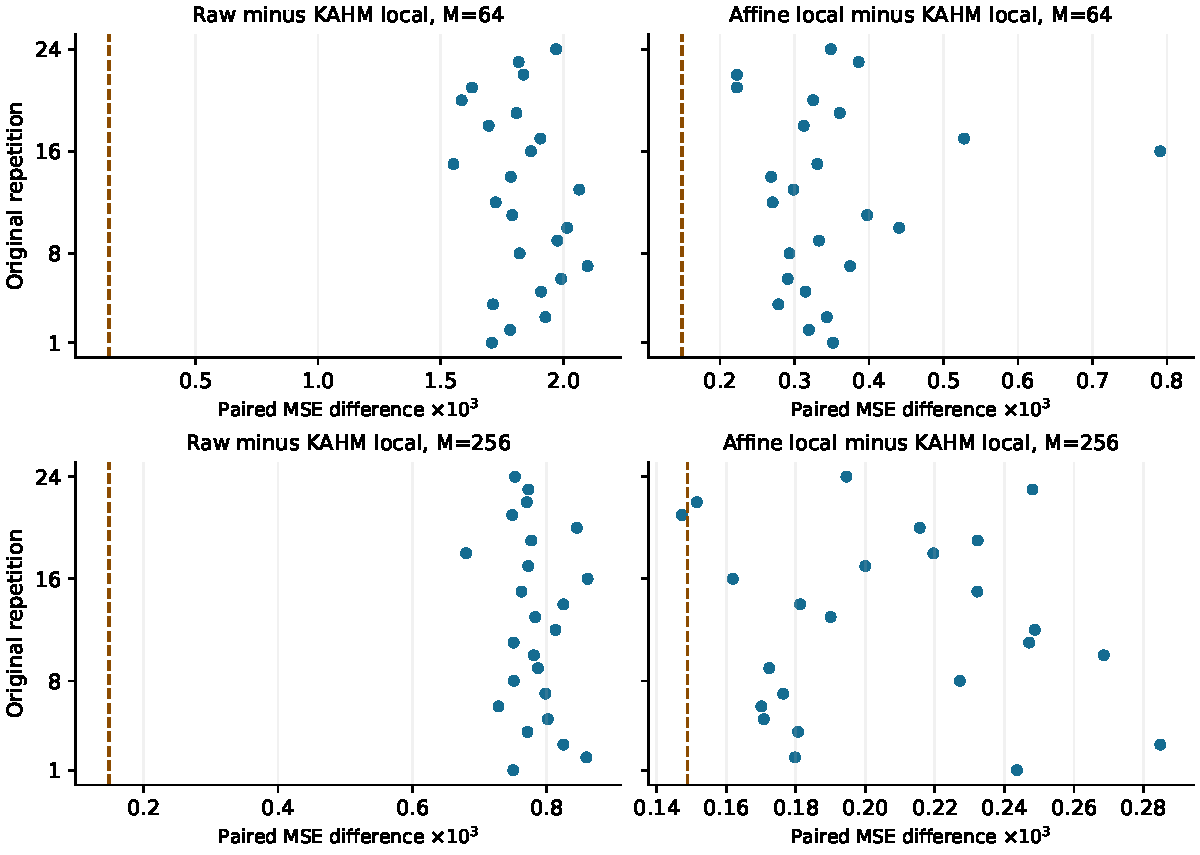
\includegraphics[width=.96\textwidth]{generated/figures/review_paired_differences.pdf}
\caption{The 24 original paired differences for each Van der Pol capacity comparison,
in units of $10^{-3}$ MSE. The dashed line is the frozen practical margin.
No resampling, refitting, or new primary analysis is performed.}
\label{fig:review-paired}
\end{figure}

We also inspect the 120 first-stage primary banks and 72 capacity banks from a
completed computational reproduction using the published seeds. No bank or head is
refitted for these diagnostics. Replayed test inputs, targets, and groups are checked
against their recorded hashes before the original feature map is evaluated.
Let $A$ vertically stack the $P_c^\top$ matrices. Proposition~\ref{prop:local-injectivity}
shows that positive gates and full column rank of $A$ suffice to recover the scaled
input from the gated local coordinates and gates:
division by $\phi_c$ recovers $P_c^\top(z-\mu_c)$, after which one solves for $z$.
A deficient stack does not establish information loss in the full code, because the
gates can carry additional information. Numerical ranks use the threshold
$\sigma_1\max\{\text{rows}(A),d\}\epsilon_{64}$; they are finite-precision diagnostics,
not exact rank proofs. Small singular values and small gates can make coordinate
recovery sensitive to perturbations. Test-sample gate minima are not population
lower bounds, and these computations do not guarantee a well-conditioned inverse
or easy decoding by any particular fitted head.
\begin{table}[htbp]
\caption{Retrospective diagnostics over 24 stored banks per row. Rank ranges concern
the stacked local bases in input dimension $d$. The smallest singular value and
gate entries are minima over the inspected banks (and, for gates, their original
test observations); $\kappa_2$ is the largest stack condition number. A dash means
that not every stack in that row has full numerical column rank. KAHM and affine
representations share the basis stack. Computational reproduction supplies no new
independent statistical replications.}
\label{tab:review-banks}
\centering\small\setlength{\tabcolsep}{3pt}
% Full column rank is sufficient; numerical ranks are diagnostics, not exact proofs.
\begin{tabular}{llrrrr}
\toprule
Phase / setting & Rank / $d$ & Min. $\sigma_d$ & Max. $\kappa_2$ & Min. $\phi^{\K}$ & Min. $\phi^{\A}$ \\
\midrule
First: Straight branch & 1/2 & $0$ & --- & $3.36\times10^{-25}$ & $2.56\times10^{-20}$ \\
First: Curved branch & 2/2 & $2.19\times10^{0}$ & $1.39\times10^{0}$ & $3.55\times10^{-28}$ & $8.97\times10^{-29}$ \\
First: Nonlinear AR & 12/12 & $6.20\times10^{-2}$ & $4.90\times10^{1}$ & $2.21\times10^{-35}$ & $2.36\times10^{-34}$ \\
First: Van der Pol & 12/12 & $1.60\times10^{-2}$ & $2.20\times10^{2}$ & $2.84\times10^{-45}$ & $9.43\times10^{-20}$ \\
First: Duffing & 12/12 & $1.33\times10^{-2}$ & $2.80\times10^{2}$ & $3.92\times10^{-43}$ & $3.11\times10^{-7}$ \\
Capacity: Nonlinear AR & 12/12 & $7.31\times10^{-2}$ & $4.19\times10^{1}$ & $9.97\times10^{-37}$ & $7.75\times10^{-37}$ \\
Capacity: Van der Pol & 12/12 & $1.60\times10^{-2}$ & $2.19\times10^{2}$ & $6.21\times10^{-44}$ & $1.56\times10^{-16}$ \\
Capacity: Duffing & 12/12 & $1.32\times10^{-2}$ & $2.84\times10^{2}$ & $5.38\times10^{-43}$ & $1.86\times10^{-8}$ \\
\bottomrule
\end{tabular}

\end{table}


\clearpage
\section{Additional Source-Derived Tables}\label{app:tables}

Tables~\ref{tab:reconstruction-details} and
\ref{tab:reflection-details} give descriptive input-geometry summaries.
The two complete primary comparison families follow. Their values
are generated from the archived outcomes, with each difference,
standard error, interval, and frozen margin independently recomputed
by the paper-asset script before it writes these tables.

\begin{table}[!htbp]
 \caption{Held-out reconstruction errors per standardized input coordinate,
 averaged over the three blocks and 24 full repetitions. ``Best'' takes
 the best local reconstruction separately in each block; ``weighted''
 averages the individual squared errors with that method's affinities.
 The affine value is lower in all 24 repetitions of each of these five
 input settings, for both summaries. These are descriptive diagnostics,
 not the supervised primary endpoint.}
 \label{tab:reconstruction-details}
 \centering\small\setlength{\tabcolsep}{4pt}
 % Generated by scripts/build_paper_assets.py; do not edit.
\begin{tabular}{lrrrr}
\toprule
Setting & KAHM best & Affine best & KAHM weighted & Affine weighted \\
\midrule
Branch $c=0$ & $3.276\times10^{-3}$ & $2.156\times10^{-16}$ & $4.006\times10^{-3}$ & $1.548\times10^{-8}$ \\
Branch $c=1$ & $3.583\times10^{-2}$ & $2.932\times10^{-2}$ & $3.793\times10^{-2}$ & $3.238\times10^{-2}$ \\
Nonlinear AR & $1.166\times10^{-2}$ & $1.084\times10^{-2}$ & $1.305\times10^{-2}$ & $1.214\times10^{-2}$ \\
Van der Pol & $4.353\times10^{-3}$ & $1.683\times10^{-3}$ & $4.495\times10^{-3}$ & $1.916\times10^{-3}$ \\
Duffing & $4.877\times10^{-3}$ & $5.613\times10^{-4}$ & $5.239\times10^{-3}$ & $1.226\times10^{-3}$ \\
\bottomrule
\end{tabular}

\end{table}

\begin{table}[!htbp]
 \caption{Branch reflection differences at training size 1,024, averaged
 over 24 banks. The statistic is a per-coordinate RMS, with and without
 training-only coordinate scaling. The raw reflection precedes the
 frozen pipeline. These values neither establish exact information
 loss for the learned code nor certify a decoder-specific population
 risk bound.}
 \label{tab:reflection-details}
 \centering\small\setlength{\tabcolsep}{5pt}
 % Generated by scripts/build_paper_assets.py; do not edit.
\begin{tabular}{rlrr}
\toprule
$c$ & Encoding & Stored-coordinate RMS & Standardized RMS \\
\midrule
0 & KAHM $\phi$ & $4.894\times10^{-1}$ & $1.402\times10^{0}$ \\
0 & Affine $\phi$ & $1.451\times10^{-9}$ & $7.533\times10^{-9}$ \\
0 & KAHM local & $5.289\times10^{-1}$ & $1.418\times10^{0}$ \\
0 & Affine local & $4.993\times10^{-1}$ & $1.236\times10^{0}$ \\
1 & KAHM $\phi$ & $5.380\times10^{-1}$ & $1.427\times10^{0}$ \\
1 & Affine $\phi$ & $5.321\times10^{-1}$ & $1.471\times10^{0}$ \\
1 & KAHM local & $4.854\times10^{-1}$ & $1.442\times10^{0}$ \\
1 & Affine local & $5.522\times10^{-1}$ & $1.473\times10^{0}$ \\
\bottomrule
\end{tabular}

\end{table}

\begin{table}[!htbp]
 \caption{Complete representation means in the fresh capacity study,
 with MSE multiplied by $10^3$. The full-score KAHM representation is
 a prespecified secondary control. These point estimates do not add
 hypotheses to the 12-comparison primary family.}
 \label{tab:capacity-means-details}
 \centering\small\setlength{\tabcolsep}{4pt}
 % Generated by scripts/build_paper_assets.py; do not edit.
\begin{tabular}{lrrrrr}
\toprule
System & $M$ & Raw & Affine local & KAHM local & KAHM scores \\
\midrule
Nonlinear AR & 64 & 4.4238 & 4.9120 & 4.8795 & 4.7984 \\
Nonlinear AR & 256 & 4.6958 & 5.2347 & 5.1749 & 4.8256 \\
Van der Pol & 64 & 2.8586 & 1.3767 & 1.0266 & 1.5711 \\
Van der Pol & 256 & 1.6541 & 1.0780 & 0.8720 & 1.0499 \\
Duffing & 64 & 3.4597 & 3.0549 & 4.2154 & 4.7005 \\
Duffing & 256 & 2.8364 & 2.7981 & 4.0736 & 3.3808 \\
\bottomrule
\end{tabular}

\end{table}

\clearpage
\subsection{Selected pipelines and realized dimensions}

The validation-selected pipeline and the retained nonlinear basis are
distinct summaries: the former describes the operational model choice,
whereas the latter records the realized dimensions behind the nominal
landmark budgets.

\begin{table}[!htbp]
 \caption{Secondary validation-only selection among the eight complete
 capacity-study pipelines. Mean test MSE is multiplied by $10^3$.
 Counts concern independent complete repetitions under each generator,
 not a new population of forecasting tasks.}
 \label{tab:capacity-selector-details}
 \centering\small\setlength{\tabcolsep}{4pt}
 % Generated by scripts/build_paper_assets.py; do not edit.
\begin{tabular}{lrl}
\toprule
System & Selector MSE & Validation selections \\
\midrule
Nonlinear AR & 4.4238 & Raw, 64: 24/24 \\
Van der Pol & 0.8720 & KAHM local, 256: 24/24 \\
Duffing & 2.7923 & Affine local, 256: 23/24; Raw, 256: 1/24 \\
\bottomrule
\end{tabular}

\end{table}

\begin{table}[!htbp]
 \caption{Retained RBF-plus-linear dimensions after the Nystr\"om
 eigenvalue cutoff in the fresh capacity study. Means and ranges cover
 the 24 repetitions in each cell. The same landmark count $M$ does not
 imply the same realized dimension or function class.}
 \label{tab:capacity-dimensions-details}
 \centering\small\setlength{\tabcolsep}{5pt}
 % Generated by scripts/build_paper_assets.py; do not edit.
\begin{tabular}{lrlrr}
\toprule
System & $M$ & Representation & Mean dimension & Range \\
\midrule
Nonlinear AR & 64 & Raw & 74.88 & 61--76 \\
Nonlinear AR & 64 & Affine local & 106.00 & 106--106 \\
Nonlinear AR & 64 & KAHM local & 106.00 & 106--106 \\
Nonlinear AR & 64 & KAHM scores & 76.71 & 62--78 \\
Nonlinear AR & 256 & Raw & 189.04 & 78--268 \\
Nonlinear AR & 256 & Affine local & 297.62 & 296--298 \\
Nonlinear AR & 256 & KAHM local & 297.50 & 293--298 \\
Nonlinear AR & 256 & KAHM scores & 148.88 & 77--219 \\
Van der Pol & 64 & Raw & 76.00 & 76--76 \\
Van der Pol & 64 & Affine local & 106.00 & 106--106 \\
Van der Pol & 64 & KAHM local & 106.00 & 106--106 \\
Van der Pol & 64 & KAHM scores & 78.00 & 78--78 \\
Van der Pol & 256 & Raw & 268.00 & 268--268 \\
Van der Pol & 256 & Affine local & 298.00 & 298--298 \\
Van der Pol & 256 & KAHM local & 272.38 & 261--285 \\
Van der Pol & 256 & KAHM scores & 231.88 & 215--251 \\
Duffing & 64 & Raw & 76.00 & 76--76 \\
Duffing & 64 & Affine local & 106.00 & 106--106 \\
Duffing & 64 & KAHM local & 105.46 & 98--106 \\
Duffing & 64 & KAHM scores & 77.96 & 77--78 \\
Duffing & 256 & Raw & 268.00 & 268--268 \\
Duffing & 256 & Affine local & 296.92 & 272--298 \\
Duffing & 256 & KAHM local & 240.38 & 176--298 \\
Duffing & 256 & KAHM scores & 214.33 & 164--270 \\
\bottomrule
\end{tabular}

\end{table}

\clearpage
% Generated; this file owns its longtable environment.
\begingroup\small\setlength{\tabcolsep}{3pt}
\begin{longtable}{llrrrl}
\caption{Complete first-stage family (29 contrasts), in original MSE units. Intervals use the two-sided 95\% Bonferroni paired-replicate Student procedure with 23 degrees of freedom. Under paired normality, each t interval is exact and Bonferroni family coverage is at least 95\%; otherwise coverage is approximate. The two stages have separate families.}\label{tab:all-stageone}\\
\toprule
Setting / budget & Contrast & $\overline D$ & Simultaneous interval & $\delta$ & Assessment \\
\midrule
\endfirsthead
\toprule
Setting / budget & Contrast & $\overline D$ & Simultaneous interval & $\delta$ & Assessment \\
\midrule
\endhead
\bottomrule\endfoot
$c=0,\lambda=0$ & $G$ & -0.000013 & $[-0.000031,\,0.000005]$ & 0.000168 & unresolved $\dagger$ \\
$c=0,\lambda=0$ & $N$ & -0.000008 & $[-0.000016,\,\ensuremath{-1.85\times10^{-7}}]$ & 0.000168 & negative $\dagger$ \\
$c=0,\lambda=0$ & $L$ & -0.000031 & $[-0.000043,\,-0.000020]$ & 0.000168 & negative $\dagger$ \\
$c=0,\lambda=0.5$ & $G$ & 0.489453 & $[0.481962,\,0.496944]$ & 0.000168 & practical + \\
$c=0,\lambda=0.5$ & $N$ & 0.000944 & $[0.000088,\,0.001799]$ & 0.000168 & positive \\
$c=0,\lambda=0.5$ & $L$ & 0.010616 & $[0.010033,\,0.011200]$ & 0.000168 & practical + \\
$c=0,\lambda=1$ & $G$ & 0.978026 & $[0.962552,\,0.993500]$ & 0.000168 & practical + \\
$c=0,\lambda=1$ & $N$ & 0.001938 & $[0.000255,\,0.003621]$ & 0.000168 & practical + \\
$c=0,\lambda=1$ & $L$ & 0.021287 & $[0.020199,\,0.022376]$ & 0.000168 & practical + \\
$c=1,\lambda=0$ & $G$ & 0.001761 & $[-0.071260,\,0.074781]$ & 0.033542 & unresolved \\
$c=1,\lambda=0$ & $N$ & 0.069128 & $[0.028663,\,0.109593]$ & 0.033542 & positive \\
$c=1,\lambda=0$ & $L$ & 0.263144 & $[0.217187,\,0.309101]$ & 0.033542 & practical + \\
$c=1,\lambda=0.5$ & $G$ & -0.004395 & $[-0.043672,\,0.034882]$ & 0.016863 & unresolved \\
$c=1,\lambda=0.5$ & $N$ & 0.040663 & $[0.019789,\,0.061538]$ & 0.016863 & practical + \\
$c=1,\lambda=0.5$ & $L$ & 0.154710 & $[0.122867,\,0.186552]$ & 0.016863 & practical + \\
$c=1,\lambda=1$ & $G$ & 0.011324 & $[0.000882,\,0.021767]$ & 0.000168 & practical + \\
$c=1,\lambda=1$ & $N$ & 0.012111 & $[0.005647,\,0.018574]$ & 0.000168 & practical + \\
$c=1,\lambda=1$ & $L$ & 0.046854 & $[0.040400,\,0.053307]$ & 0.000168 & practical + \\
Nonlinear AR & $G$ & \ensuremath{-1.89\times10^{-7}} & $[-0.000050,\,0.000049]$ & 0.000253 & unresolved $\dagger$ \\
Nonlinear AR & $N$ & -0.000016 & $[-0.000062,\,0.000029]$ & 0.000253 & unresolved $\dagger$ \\
Nonlinear AR & $L$ & 0.000433 & $[0.000368,\,0.000498]$ & 0.000253 & practical + \\
Van der Pol & $G$ & -0.049419 & $[-0.060532,\,-0.038307]$ & 0.002036 & negative \\
Van der Pol & $N$ & 0.013443 & $[0.005084,\,0.021803]$ & 0.002036 & practical + \\
Van der Pol & $L$ & 0.096633 & $[0.092436,\,0.100830]$ & 0.002036 & practical + \\
Duffing & $G$ & -0.030948 & $[-0.035414,\,-0.026482]$ & 0.000338 & negative \\
Duffing & $N$ & 0.005558 & $[0.001721,\,0.009395]$ & 0.000338 & practical + \\
Duffing & $L$ & 0.046168 & $[0.041729,\,0.050608]$ & 0.000338 & practical + \\
$c=0$ interaction & $I_0$ & -0.978039 & $[-0.993512,\,-0.962566]$ & 0.000168 & opposite sign \\
$c=1$ interaction & $I_1$ & -0.009564 & $[-0.082839,\,0.063712]$ & 0.016855 & unresolved \\
\end{longtable}
\noindent $\dagger$: the entire interval lies within the fixed practical band $[-\delta,\delta]$. An unresolved sign alone does not establish equivalence.
\endgroup

\clearpage
% Generated; this file owns its longtable environment.
\begingroup\small\setlength{\tabcolsep}{3pt}
\begin{longtable}{llrrrl}
\caption{Complete fresh capacity family (12 contrasts). All numerical loss quantities are multiplied by $10^3$. Intervals use the two-sided 95\% Bonferroni paired-replicate Student procedure with 23 degrees of freedom. Under paired normality, each t interval is exact and Bonferroni family coverage is at least 95\%; otherwise coverage is approximate. The two stages have separate families.}\label{tab:all-capacity}\\
\toprule
Setting / budget & Contrast & $\overline D$ & Simultaneous interval & $\delta$ & Assessment \\
\midrule
\endfirsthead
\toprule
Setting / budget & Contrast & $\overline D$ & Simultaneous interval & $\delta$ & Assessment \\
\midrule
\endhead
\bottomrule\endfoot
Nonlinear AR / 64 & Raw--K & -0.4556 & $[-0.5235,\,-0.3878]$ & 0.2201 & negative \\
Nonlinear AR / 64 & Affine--K & 0.0325 & $[-0.0031,\,0.0680]$ & 0.2201 & unresolved $\dagger$ \\
Nonlinear AR / 256 & Raw--K & -0.4791 & $[-0.6013,\,-0.3569]$ & 0.2201 & negative \\
Nonlinear AR / 256 & Affine--K & 0.0598 & $[-0.0131,\,0.1327]$ & 0.2201 & unresolved $\dagger$ \\
Van der Pol / 64 & Raw--K & 1.8320 & $[1.7369,\,1.9271]$ & 0.1489 & practical + \\
Van der Pol / 64 & Affine--K & 0.3501 & $[0.2755,\,0.4247]$ & 0.1489 & practical + \\
Van der Pol / 256 & Raw--K & 0.7822 & $[0.7550,\,0.8094]$ & 0.1489 & practical + \\
Van der Pol / 256 & Affine--K & 0.2060 & $[0.1810,\,0.2311]$ & 0.1489 & practical + \\
Duffing / 64 & Raw--K & -0.7557 & $[-1.0831,\,-0.4282]$ & 0.1727 & negative \\
Duffing / 64 & Affine--K & -1.1605 & $[-1.4707,\,-0.8503]$ & 0.1727 & negative \\
Duffing / 256 & Raw--K & -1.2372 & $[-1.5242,\,-0.9503]$ & 0.1727 & negative \\
Duffing / 256 & Affine--K & -1.2756 & $[-1.5702,\,-0.9810]$ & 0.1727 & negative \\
\end{longtable}
\noindent $\dagger$: the entire interval lies within the fixed practical band $[-\delta,\delta]$. An unresolved sign alone does not establish equivalence.
\endgroup

